\documentclass[11pt]{article}

\usepackage{graphicx}
\usepackage{wrapfig}
\usepackage{url}
\usepackage{wrapfig}
\usepackage{color}
\usepackage{marvosym}
\usepackage{enumerate}
\usepackage{subfigure}
\usepackage{tikz}
\usepackage{amsmath}
\usepackage{amssymb}
\usepackage{hyperref}
\usepackage{bbm}


\oddsidemargin 0mm
\evensidemargin 2mm
\topmargin -20mm
\textheight 240mm
\textwidth 160mm



\newcommand{\vwi}{{\bf w}_i}
\newcommand{\vw}{{\bf w}}
\newcommand{\vx}{{\bf x}}
\newcommand{\vy}{{\bf y}}
\newcommand{\vxi}{{\bf x}_i}
\newcommand{\yi}{y_i}
\newcommand{\vxj}{{\bf x}_j}
\newcommand{\vxn}{{\bf x}_n}
\newcommand{\yj}{y_j}
\newcommand{\ai}{\alpha_i}
\newcommand{\aj}{\alpha_j}
\newcommand{\X}{{\bf X}}
\newcommand{\Y}{{\bf Y}}
\newcommand{\vz}{{\bf z}}
\newcommand{\msigma}{{\bf \Sigma}}
\newcommand{\vmu}{{\bf \mu}}
\newcommand{\vmuk}{{\bf \mu}_k}
\newcommand{\msigmak}{{\bf \Sigma}_k}
\newcommand{\vmuj}{{\bf \mu}_j}
\newcommand{\msigmaj}{{\bf \Sigma}_j}
\newcommand{\pij}{\pi_j}
\newcommand{\pik}{\pi_k}
\newcommand{\D}{\mathcal{D}}
\newcommand{\el}{\mathcal{L}}
\newcommand{\N}{\mathcal{N}}
\newcommand{\vxij}{{\bf x}_{ij}}
\newcommand{\vt}{{\bf t}}
\newcommand{\yh}{\hat{y}}
\newcommand{\code}[1]{{\footnotesize \tt #1}}
\newcommand{\alphai}{\alpha_i}
\graphicspath{ {pic/} } 

\pagestyle{myheadings}

\title{Object-Oriented Software Design\\Assignment 2: Object-Oriented Design}
\author{Li-Yi Lin / llin34@jhu.edu}
\date{}

\begin{document}
\large
\maketitle
\thispagestyle{headings}

\section{Question 1: Fitness Center Software Design}
\paragraph{I) Feature List:}
\begin{enumerate}[(a)]
%%
\item Membership:
\begin{enumerate}[(1)]
\item Allow the center to create a new member account for a new customer.
\item Allow the center to set the membership of a member account.
\item The membership can be bought for one month, six months, and one year at a time.
\item The membership must have two kinds of memberships: basic and premium memberships.
\item Allow the center to renew a membership.
\item Allow a member to switch from basic to premium membership by paying a pro-rated membership fee.
\item Ensure switching from premium to basic is allowed only during renewal.
\item Be able to calculate the membership fee.
\item Be able to keep track of customers and their memberships including historical information.
\item Allow the center to deactivate, suspend, activate a membership.
\end{enumerate}
%%
\item Access control:
\begin{enumerate}[(1)]
\item Have access controls for facilities according to different memberships. 
\item The basic and premium memberships shall be able to access most facilities (including the weight room and the pool).
\end{enumerate}
%%
\item Personal trainer:
\begin{enumerate}[(1)]
\item Allow the premium membership to have five free appointments with a personal trainer per month.
\item Allow a member to pay small fee to get personal training appointments.
\item Be able to keep track of personal trainer appointments and avoid double-booking.
\item Be able to prevent a member from booking more than one appointments for the same time period.
\item Allow a member to cancel her/his personal trainer schedule.
\end{enumerate}
%%
\item Membership fee:
\begin{enumerate}[(1)]
\item Allow the center to update the pricing of the memberships.
\item The change in price should not affect the current memberships until it is renewed.
\item Allow members to lapse in their payments.
\item Allow members to be late up to a month without being refused entry to the fitness center. But this applies only to customers who have had a membership (continously) for at least the last six months and have not lapsed in payment during that time frame.
\item Be able to automatically suspend a membership when some conditions are met (e.g. not pay membership fee one month later after the membership expiration date).
\end{enumerate}
%If you have had a membership for more than 6 months and you have been paying correctly for the past 6 months, you get leniency. If you start paying properly again and accumulate another 6 months of good credit, you can pay late again.
\end{enumerate}

%%%%%%%%%%%%%%%%%%%%%%%%%%%%%%%%%%%%%%%%%%%%%%
\paragraph{II) Use Cases:}
(x.x means alternate path)
\begin{enumerate}[(a)]
\item Create member account:\\
1. The staff opens the "Create Account" function.\\
2. The staff fills in information about a new member.\\
3. The staff sets the membership (basic or premium) of the new account.\\
4. The staff sets the membership duration (one month, six months, or one year).\\
5. The staff clicks the "Create" button and the data is sent to backend systems.\\
6. The system replies success message.\\
\- 6.1. The system replies error message if creating account failed.
%%
% \item Add facilities:\\
% 1.The staff opens the "Manage Facility" function.\\
% 2.The staff clicks the "Add Facilities" button.\\
% 3.The staff fills in the information about new facilities.\\
% 4.The staff clicks the "Add" button and the data is sent to backend systems.\\
% 5.The system replies operation status:\\
% \- 5.1 The system replies success message.\\
% \- 5.2 The system replies error message if adding facilities failed.
% %
% \item Delete facilities:\\
% 1.The staff opens the "Manage Facility" function.\\
% 2.The staff clicks the "Facility List" button.\\
% \- 2.1 The system replies "No facility" message if there is no facility in the system.\\
% \- 2.2 The system replies a list of all facilities (divided into pages if having too many facilities).\\
% 3.If there are facilities, the staff chooses facilities to be deleted.\\
% 4.The staff clicks the "Delete" button and the data is sent to backend systems.\\
% 5.The system replies operation status:\\
% \- 5.1 The system replies success message.\\
% \- 5.2 The system replies error message if adding facilities failed.
%%
% \item Add access control type:\\
% 1.The staff opens the "Access Control" function.\\
% 2.The staff clicks the "Add Access Control List" button.\\
% 3.The staff fills in the information about the access control list.\\
% 4.The staff choose facilities for this access control list.\\
% 5.The staff clicks the "Add" button and the data is sent to the backend systems.\\
% 6.The system replies operation status:\\
% \- 6.1 The system replies success message.\\
% \- 6.2 The system replies error message if adding access control list failed.
%%
\item Query member:\\
1. The staff opens the "Manage Member" function.\\
2. The staff enter the member account in the search area and clicks the "Search" button.\\
3. The system replies member's data.\\
\- 3.1. The system replies "member not found."
%%
\item Query members' membership history:\\
Precondition: The staff has found the member using "Query member" function.\\
1. In the query member's page, the staff clicks "Membership History" button.\\
2. The system replies the result and shows the result on a membership history page.
%% 
\item Renew membership:\\
Precondition: The staff has found the member using "Query member" function.\\
1. The staff clicks the "Renew Membership" button.\\
2. The system shows that the member could renew the membership. The member can renew her/his membership only when the remainder duration of the membership is no more than one month (this is an assumption).\\
\- 2.1. If the member's status is not qualified for membership renewal, the system will show a warning message. Stop this operation.\\
3. The staff chooses a membership type (basic or premium).\\
4. The staff chooses a membership duration (one month, six months, or one year).
5. The staff clicks "Renew" button.\\
6. The system shows a page about the renewal information and asks the staff to confirm this renewal.\\
7. The staff clicks "Confirm" button and the data is sent to the backend systems.\\
8. The system replies success message.\\
\- 8.1. The system replies error message.
%%
\item Suspend a membership:\\
Precondition: The staff has found the member using "Query member" function and the member's status is neither suspended nor inactive.\\
1. The staff clicks "Change Member Status" button and the system shows a status management page.\\
2. The staff chooses a new status for this member and enters a reason for this change (could select from a reason list).\\
3. The staff clicks "Change" button.\\
4. The system shows a confirmation page and the staff clicks "Confirm" button.\\
5. The system replies success message.\\
\- 5.1. The system replies error message.
%%
\item Deactivate a membership:\\
Precondition: The staff has found the member using "Query member" function and the member's status is not inactive.\\
1. The staff clicks "Change Member Status" button and the system shows a status management page.\\
2. The staff chooses a new status for this member and enters a reason for this change (could select from a reason list).\\
3. The staff clicks "Change" button.\\
4. The system shows a confirmation page and the staff clicks "Confirm" button.\\
5. The system replies success message.\\
\- 5.1. The system replies error message.
%%
\item Switch membership type:\\
Precondition: The staff has found the member using "Query member" function and the membership type is basic and the member status is "current".\\
1. The staff clicks "Switch Membership Type" button and the system shows a new page for switching membership type.\\
\- 1.1. If the current status of the member is not suitable for swithcing membership type, the system will show a warning message. Stop this operation.\\ 
2. The staff chooses a new membership type for this member.\\
3. The staff clicks "Switch" button.\\
4. The system shows a confirmation page and the staff clicks "Confirm" button.\\
5. The system replies success message.\\
\- 5.1. The system replies error message.
%%
\item Book personal Trainer:\\
Precondition: The staff has found the member using "Query member" function and the member status is "current."\\
1. The staff clicks "Book Personal Trainer" button and the system shows a page for booking personal trainer.\\
2. The staff choose a time slot.\\
3. The staff choose a personal trainer if available.\\
\- 3.1 There is no personal trainer available. Go back to step 2 and choose another time slot.\\
4. The staff clicks "Create" button.\\
5. The system shows a confirmation page.\\
\- 5.1 The system shows error message if the member has no enough personal trainer quota to use. Stop this operation.\\
6. The staff clicks "Confirm" button.\\
7. The system replies success message and the personal trainer hours will be substracted from the member's account.\\
\- 7.1 The system replies error message.
%%
\item Cancel personal trainer schedule:\\
Precondition: The staff has found the member using "Query member" function.\\
1. The staff clicks "Personal Trainer Schedule" button and the system shows a page of the member's schedules for personal trainer.\\
2. The staff choose a unexpired schedule and the system shows a page about this detailed personal trainer schedule.\\
\- 3.1 There is no personal trainer available. Go back to step 2 and choose another time slot.\\
4. The staff clicks "Create" button.\\
5. The system shows a confirmation page.\\
\- 5.1 The system shows error message if the member has no enough personal trainer quota to use. Stop this operation.\\
6. The staff clicks "Confirm" button.\\
7. The system replies success message and the personal trainer hours will be added back to the member's account.\\
\- 7.1 The system replies error message.
%%
\item Pay for personal trainer:\\
Precondition: The staff has found the member using "Query member" function and the member status is "current."\\
1. The staff clicks "Add Personal Trainer Hour" button and the system shows a new page for adding hours for this member.\\
\- 1.1. If the member status is not suitable for this operation, the system will show a warning message. Stop this operation.\\ 
2. The staff enters the number of hours the member want to add for the personal trainer.\\
3. The system shows the total amount of fee the member should pay for it.\\
4. The staff clicks "Add" button.\\
5. The system shows a confirmation page and the staff clicks "Confirm" button.\\
5. The system replies success message and the personal trainer hours will be added to the member's account.\\
\- 5.1. The system replies error message.
%%
\item Update the pricing of the memberships:\\
1. The staff clicks "Membership Configuration" button and the system shows a new page for configuring membership setting.\\
2. The staff clicks "Membership Pricing" button and the system shows a new page for changing membership pricing.\\
3. The staff enter a new membership pricing for the membership she/he want to change.\\
4. The staff clicks "Update" button.\\
5. The system shows a confirmation page and the staff clicks "Confirm" button.\\
6. The system replies success message.\\
\- 6.1 The system replies error message.
%%
\end{enumerate}
%%%%%%%%%%%%%%%%%%%%%%%%%%%%%%%%%%%%%%%%%%%%%%
\paragraph{III) State Diagram:\\}
\begin{center}
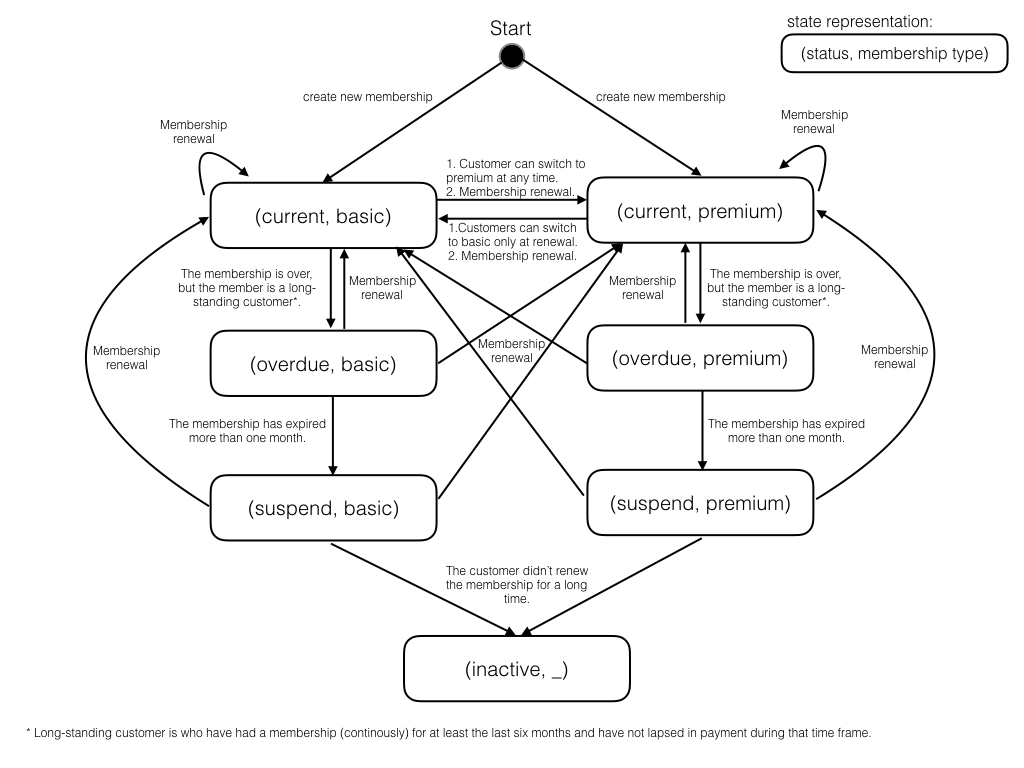
\includegraphics[scale=0.5]{StateDiagram.jpeg} 
\end{center}

%%%%%%%%%%%%%%%%%%%%%%%%%%%%%%%%%%%%%%%%%%%%%%
\newpage
\paragraph{IV) UML Class Diagram:\\}
\begin{center}
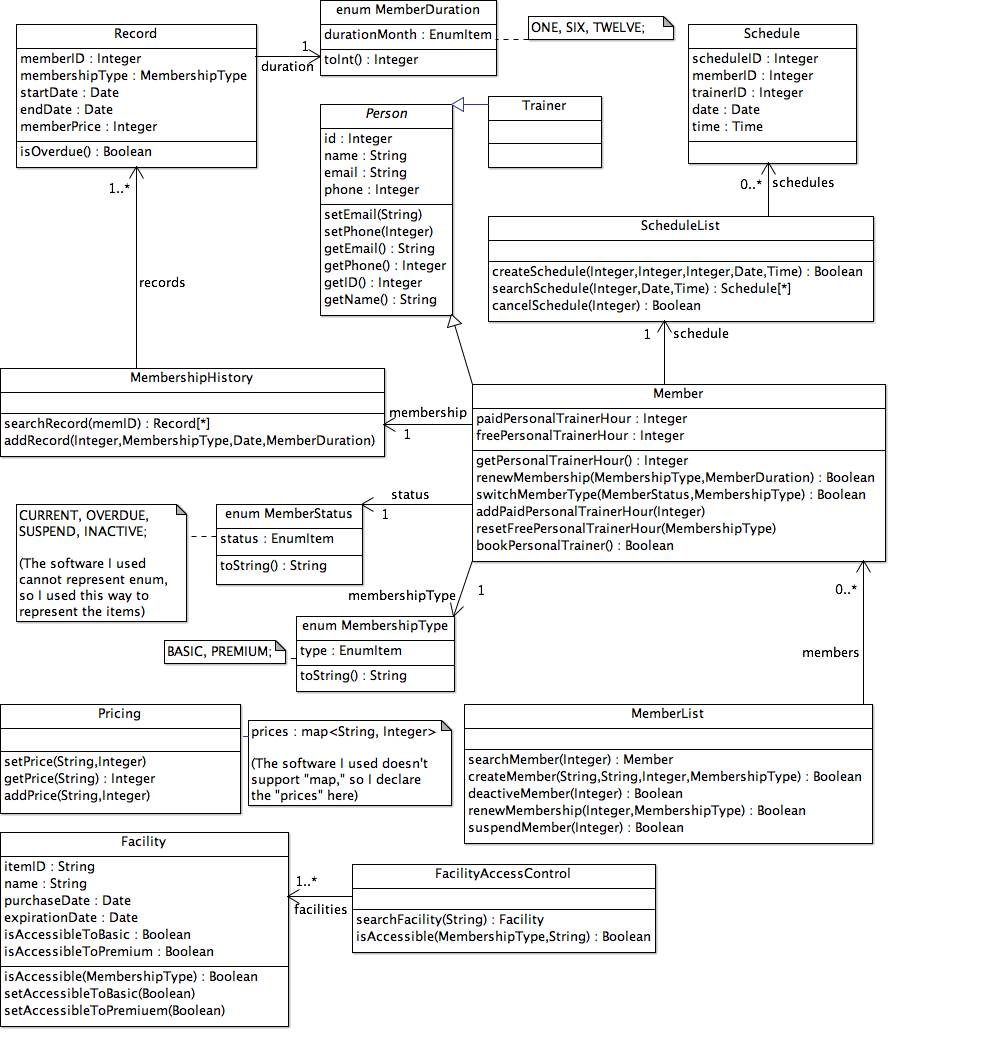
\includegraphics[scale=0.5]{ClassDiagram} 
\end{center}

%%%%%%%%%%%%%%%%%%%%%%%%%%%%%%%%%%%%%%%%%%%%%%
\paragraph{V) Extended Requirements:\\}
\begin{enumerate}
\item The system can allow the center to manage facilities.
\item The system can allow the center to change the access control for different kinds of memberships.
\item The system can allow the center to manage the personal trainers' information.
\item The system can allow the center to manage the time slots of personal trainers.
\item The system can automatically renew the membership if the member provides her/his credit card information and permit the center to do so. 
\item The system can repeat the personal trainer schedule periodically for members.
\item The system can send personal trainer schedule reminder (using SMS or email) to members.
\item The system can a have a member page for members to reserve the personal trainer online.

\end{enumerate}
%%
\newpage
\section{Question 2: Object-Oriented Design Principles}
\textbf{Case 1:}\\
In case 1, the code violates the "Liskov Substitution Principle (LSP)" because when "MyMultiSet" class is replaced with its subclass "Set," the result of calling "add" method will be different. The "add" method of "MyMultiSet" will always add the item into its list "data." However, the subclass "Set" will add a new itme into its list "data" only when its list "data" has no item equals to the new item. In some cases, the subclass will override the method inherited from its superclass on purpose (like the "add" method in "Set"). If we really want to correct the code so that it will not violate LSP, we can change the method name of "add" in class "Set" to another name so that when "MyMultiSet" is replaced with subclass "Set", the result will not change.\\
This case could also be "Open Close Principle (OCP)" violation because subclass can modify the superclass' methods. To close the superclass' methods for modification, we can declare its methods as "final."\\

%%%
\noindent
\textbf{Case 2:}\\
In case 2, the code violates the "Don't Repeat Youself (DRY)" principle. The actions of "slashWithSword(Monster target)" and "pokeWithSpear(Monster target)" are almost the same except the calculation of differenet damages. This DRY violation can be corrected if we calculate the damage value according to different weapon types in the switch section. After the switch section, add "target.addDamage(damage);" before the end of the "attack" method. So the code will become\\

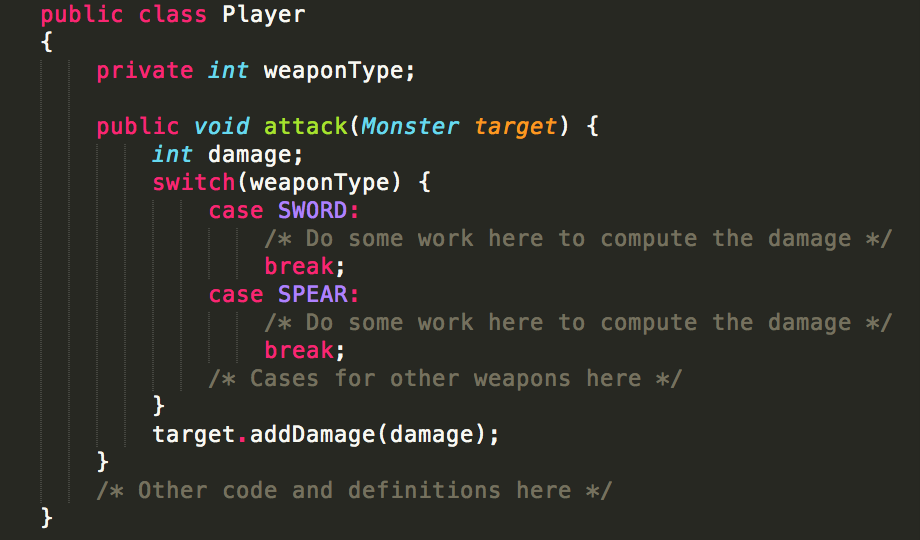
\includegraphics[scale=0.8]{case2_1}\\

Thus, the "slashWithSword(Monster target)" and "pokeWithSpear(Monster target)" methods can be deleted. Furthermore, if the damage calculations are very similiar between different weapon types, we can create a new method to calculate the damage value according to different parameters. The code will become\\

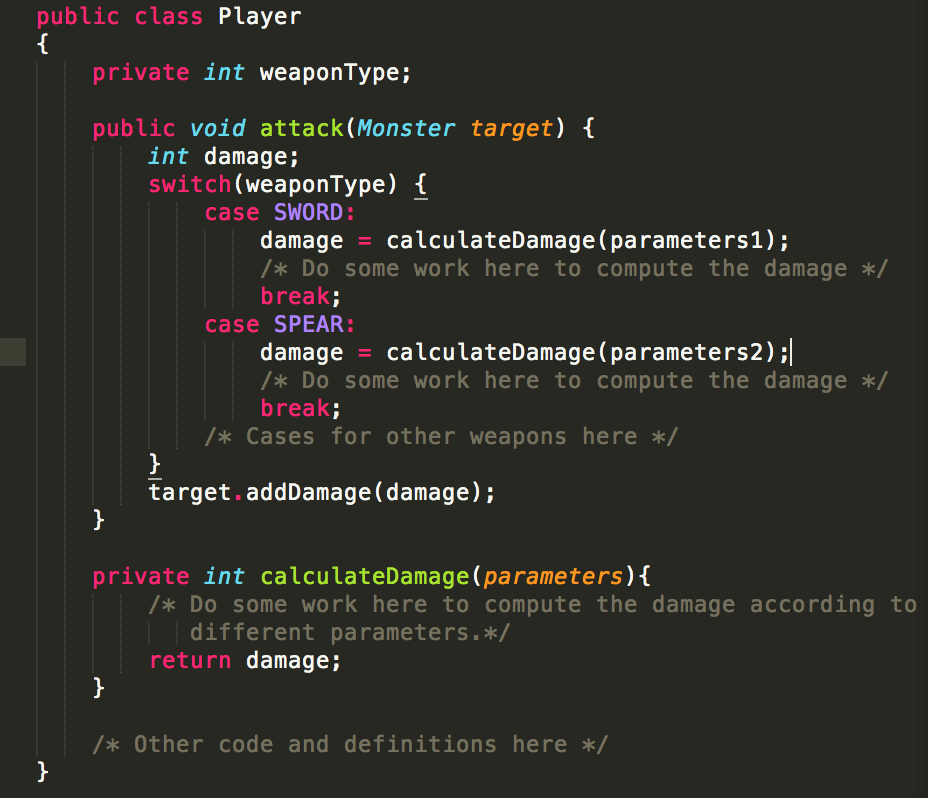
\includegraphics[scale=0.8]{case2_2}\\
%%%

\noindent
\textbf{Case 3:}\\
In case 3, the code violates the "Single Responsibility Principle (SRP)" because the "Game" class are responsible for getting user input, moving a piece, and printing the board, which are not necessarily the responsibilities the "Game" class should do. To correct the SRP violation, we can create a "Board" class that deals with moving pieces and printing the board. And the "Game" class deals with getting user input and interacting with the "Board" class. Therefore, each class can focus on the responsibilities it should do.\\

%%%
\noindent
\textbf{Case 4:}\\
In case 4, we assume the "Game" class is responsible for moving a piece. The code violates the "Don't Repeat Youself (DRY)" principle because it lists all the ckecks for all the possible moves for a piece. This will create many duplicate codes. To correct the DRY violation, it should analyze the possible moves and simplify the checks. To simplify the checks, it should first check a rule that will reduce following checks as much as possible and so on. By doing so, the move check will become much simpler and will not have duplicate codes.


\end{document}
